% Full title as you would like it to appear on the page
\chapter{Interpolating The Global Wavefront with Least Squares}
\label{chap:interp}
\chaptermark{Interpolating The Global Wavefront}

\epigraph{In questions of science, the authority of a thousand is not worth the humble reasoning of a single individual.}{Galileo Galilei}
% \epigraph{The first principle is that you must not fool yourself and you are the easiest person to fool.}{Richard P. Feynman}

\section{The Interpolation Geometry}

In the second step, we interpolate the global wavefront from the local wavefront predictions from the first step. We interpolate the global wavefront coefficients $\beta_{jk}$ based on the predictions $\alpha$ from the previous step. More explicitly, we use ordinary least squares (LS) to solve

\begin{equation*}
\text{LS}(\alpha(x_1,y_1), \dots, \alpha(x_n,y_n)) \to \beta_{jk} \text{ such that } W(u,v,x,y) = \sum_{j=4}^{21}\sum_{k=1}^3\beta_{jk}Z_j(u,v)Z_k(x,y)
\end{equation*}

In the previous step, the 18 predictions $\{\alpha_4(x_i, y_i), \dots, \alpha_{21}(x_i,y_i)\}$ for a source image $D$ at position $(x_i,y_i)$. In this step, we start by aggregating the predictions for a single coefficient $j$ for all $n$ donuts in the field of view of the observation, or $\{\alpha_j(x_1, y_1), \dots, \alpha_{j}(x_n,y_n)\}$. Then the problem reduces to minimizing the distance between the $\alpha_j$ estimates and $\sum_{k=1}^3\beta_{jk}Z_k(x,y)$ for each index separately. Figure \ref{fig:rafts} shows the true and predicted $\alpha_4$ values on the four wavefront sensors. 

\begin{figure}[!htbp]
\begin{center}
\begin{tabular}{c}
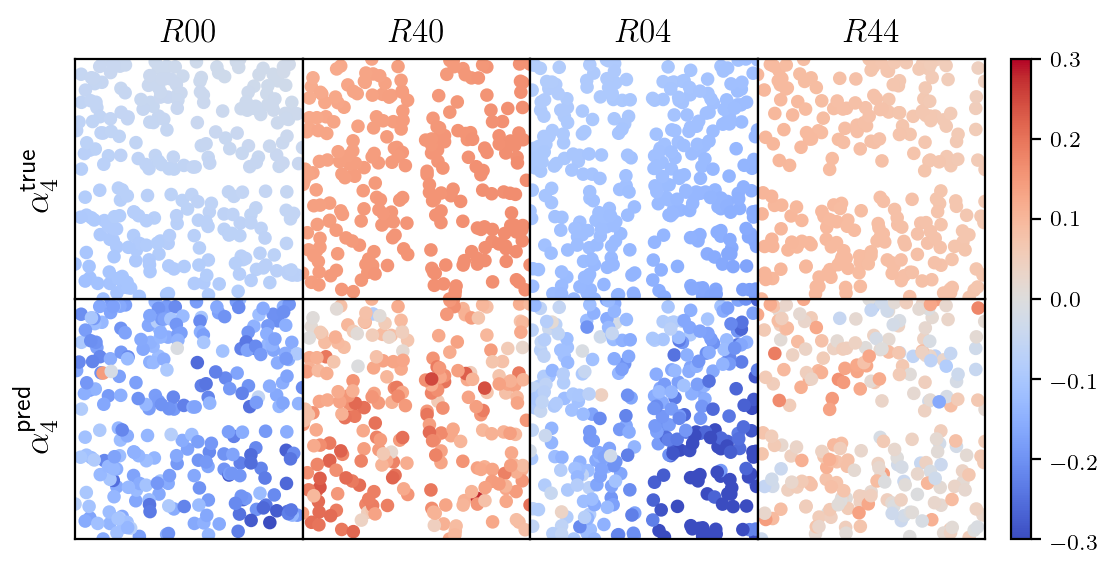
\includegraphics[width=\textwidth]{figs/interp/rafts.png}
\end{tabular}
\end{center}
\caption[Local Wavefront Predictions Across Four Wavefront Sensors]{The two rows correspond to the true ($\alpha_4^{\text{true}}$) and predicted ($\alpha_4^{\text{predicted}}$) $Z_4$ coefficients. The four columns correspond to the four corner wavefront sensors. The colormap is in units of waves.\label{fig:rafts}}
\end{figure}

The first three Zernike coefficients establish a plane. Thus we are effectively fitting a plane by the three coefficients along the $k$ index, for each local wavefront Zernike coefficient, or $j$ index. Figure \ref{fig:fieldols} shows how $\beta_{41}, \beta_{42}, \beta_{43}$ are fit from the local $\alpha_4$ predictions.

\begin{figure}[!htbp]
\begin{center}
\begin{tabular}{c}
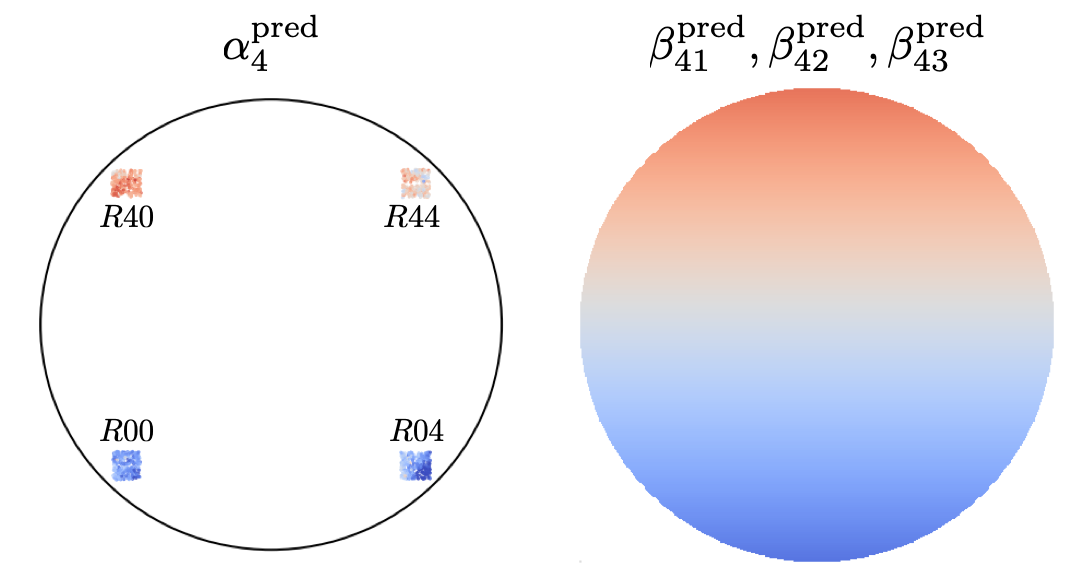
\includegraphics[width=\textwidth]{figs/interp/fieldols.png}
\end{tabular}
\end{center}
\caption[Fitting Global $\beta_{41}, \beta_{42}, \beta_{43}$ From Local $\alpha_4$ Predictions]{\textit{Left:} the predicted coefficients $\alpha_4^{\text{pred}}$ from Figure \ref{fig:rafts} shown at their corresponding field locations within the field of view. \textit{Right:} the plane characterized by the three fit double Zernike coefficients $\beta^{\text{pred}}_{41},\beta^{\text{pred}}_{42}, \beta^{\text{pred}}_{43}$. The two circles represent the field of view of the Rubin Observatory. \label{fig:ls-intuition}}
\end{figure}

The explicit minimization is 

\begin{equation*}
\label{eq:objective}
\text{min}_{\beta}\left|\left| \begin{bmatrix}\alpha_j(x_1,y_1) \\ \vdots \\ \alpha_j(x_n,y_n) \end{bmatrix} - \begin{bmatrix}Z_1(x_1,y_1) & Z_2(x_1,y_1) & Z_3(x_1,y_1) \\ \vdots & \vdots & \vdots\\  Z_1(x_n,y_n) & Z_2(x_n,y_n) & Z_3(x_n,y_n)\end{bmatrix} \begin{bmatrix}\beta_{j1} \\ \beta_{j2} \\ \beta_{j3} \end{bmatrix}\right|\right|_2
\end{equation*}

\noindent which we solve with ordinary least squares. Letting $\alpha_j, Z, \beta_j$ be the vectors and matrices from the equation above, we have the analytic solution $\beta_j = (Z^TZ)^{-1}Z^T\alpha_j$. After solving this equation for each $j$, we have $\beta_{jk}$ for $4 \leq j \leq 21$ and $1 \leq k \leq 3$. In the next section we describe a few variations to this basic framework.

\section{Evaluating Different Interpolation Strategies}

The interpolation is comprised of three steps that are reminiscent of a standard data query: select, reduce, and fit. The \textit{select} step decides which donuts and corresponding local estimates to use in the interpolation. The \textit{reduce} step, which is typically skipped, reduces these estimates across a wavefront sensor. The \textit{fit} step fits the local coefficients to a global Zernike basis based on the provided loss function.

We examine multiple variations in each of these steps to find which combination works best. We explore selecting donuts from all the sources (stars and blends), from only the non-blended stars (stars), the non-blended 10 brightest stars per chip (brightest stars), and using the true labels (labels). The results on the true labels provide a sanity check and bound the performance we can expect to achieve with alternatives. 

We also analyze two variations in the reduce step. Either we make no changes to estimates and effectively skip this step, or we take the median of the estimates on each chip. In the median case, we would then fit against the four points corresponding to the four sensors in the fit step. 

We explore three different fitting strategies. The $\ell_1$, or absolute loss, is convex and can be found with an iterative optimization algorithm. The $\ell_2$, or least squares loss, has an analytic solution. This has the added benefit of making error propagation analytic as well. Finally, the Huber loss $\ell_h$ is similar to the $\ell_2$ for samples with small error but scales like $\ell_1$ for large error. Thus it is similar to $\ell_2$ but less sensitive to outliers.

The results of these variations, applied to the local wavefront estimates from the neural network, applied to the full visit dataset, are shown in Table \ref{tab:variations}. We compare the true global wavefront and the residual global wavefront, where the residual is the true wavefront minus the interpolated optics wavefront. The residual wavefront is smaller than the original wavefront for all the samples in the majority of select-reduce-fit variations. The consistency of the improvements makes our method an attractive candidate for deployment.

\begin{table}
{
\begin{center}
\begin{tabular}{|c|c|c|c|r|}
\hline
 & Median &  & \multicolumn{1}{|c|}{\% Samples} & \multicolumn{1}{|c|}{Relative}  \\
Select & Reduce & Fit & \multicolumn{1}{|c|}{Improved} & \multicolumn{1}{|c|}{Residual} \\
\hline
 &  & $\ell_1$ & $ 99.6$ & $ 0.48 \pm  0.13$\\
Stars & & $\ell_2$ &  $ 99.8$ & $ 0.49 \pm  0.12$\\
and&  & $\ell_{\text{h}}$ &  $ 100.0$ & $ 0.48 \pm  0.12$\\
Blends& \checkmark & $\ell_{1}$ &  $ 97.8$ & $ 0.67 \pm  0.14$\\
& \checkmark & $\ell_{2}$ &  $ 100.0$ & $ 0.46 \pm  0.12$\\ 
\hline
&   & $\ell_1$ &  $ 99.8$ & $ 0.44 \pm  0.11$\\ 
&   & $\ell_2$ &  $ 100.0$ & $ 0.43 \pm  0.10$\\ 
Stars&  & $\ell_{\text{h}}$ &  $ 100.0$ & $ 0.43 \pm  0.10$\\
& \checkmark  & $\ell_{1}$ &  $ 97.2$ & $ 0.64 \pm  0.14$\\
& \checkmark  & $\ell_{2}$ &  $ 99.8$ & $ 0.41 \pm  0.11$\\
\hline
& & $\ell_1$ &  $ 99.6$ & $ 0.37 \pm  0.13$\\ 
Brightest& & \textcolor{blue}{$\ell_2$} & \textcolor{blue}{$ 100.0$} & \textcolor{blue}{$ 0.34 \pm  0.12$}\\ 
Stars& & $\ell_{\text{h}}$ &  $100.0$ & $ 0.34 \pm  0.12$\\ 
& \checkmark & $\ell_{1}$ &  $97.2$ & $ 0.60 \pm  0.16$\\ 
& \checkmark & $\ell_{2}$ &  $100.0$ & $ 0.35 \pm  0.12$\\
\hline
& & $\ell_1$ &  $ 100.0$ & $ 0.13 \pm  0.05$\\ 
Labels & & \textcolor{red}{$\ell_2$} & \textcolor{red}{$ 100.0$} & \textcolor{red}{$ 0.06 \pm  0.02$}\\
& & $\ell_{\text{h}}$ &  $ 100.0$ & $ 0.08 \pm  0.04$\\ 
\hline
\end{tabular}
\end{center}
}
\caption[Select-Reduce-Fit Results]{Each row contains the results for a different combination of select, reduce, and fit steps. The penultimate column contains the percentage of the number of samples where the residual improved. The final column contains the relative residual: the total magnitude of the residual divided by the total magnitude of the true wavefront. The best variation on neural network estimates is highlighted in \textcolor{blue}{blue}. The best variation on the true label estimates is highlighted in \textcolor{red}{red}.}
\label{tab:variations}
\end{table}

This experiment also taught us that more data is not always better. Ignoring the blended donuts leads to a clear improvement in performance. So does ignoring all but the brightest stars. This suggests that we should prioritize making accurate predictions on the best donuts, perhaps at the expense of making consistent estimates on all the donuts. It also may have consequences for wavefront sensing in crowded fields where almost all of the donuts are blended.

We can also draw conclusions about the variations. Taking the median and fitting with the $\ell_1$ norm appears to discard too much information. We also see that the benefit of using median with the $\ell_2$ norm goes away as the select becomes more selective. This is likely because the outliers, which the median reduce suppresses, get filtered and are no longer an issue. The $\ell_{h}$ norm also seems to do comparatively well on stars and blends, but loses this advantage on the more selective brightest stars selection. We conclude using the $\ell_2$ norm, with no median reduce, to fit the brightest stars, is the best variation.

We used this variation to explore how our framework performs in five scenarios. We used the relative residual $|\beta^{\text{res}}| / |\beta^{\text{true}}| = \sum_{jk}|\beta^{\text{true}}_{jk} - \beta^{\text{pred}}_{jk}| / \sum_{jk}|\beta^{\text{true}}_{jk}|$ to measure our algorithm's capability to reproduce the true global wavefront. A value close to zero means the predictions match the true global wavefront almost perfectly; a value close to one means the predictions capture almost none of the true global wavefront. Figure \ref{fig:beta-results} shows the results.

\begin{figure}[!htbp]
\begin{center}
\begin{tabular}{c}
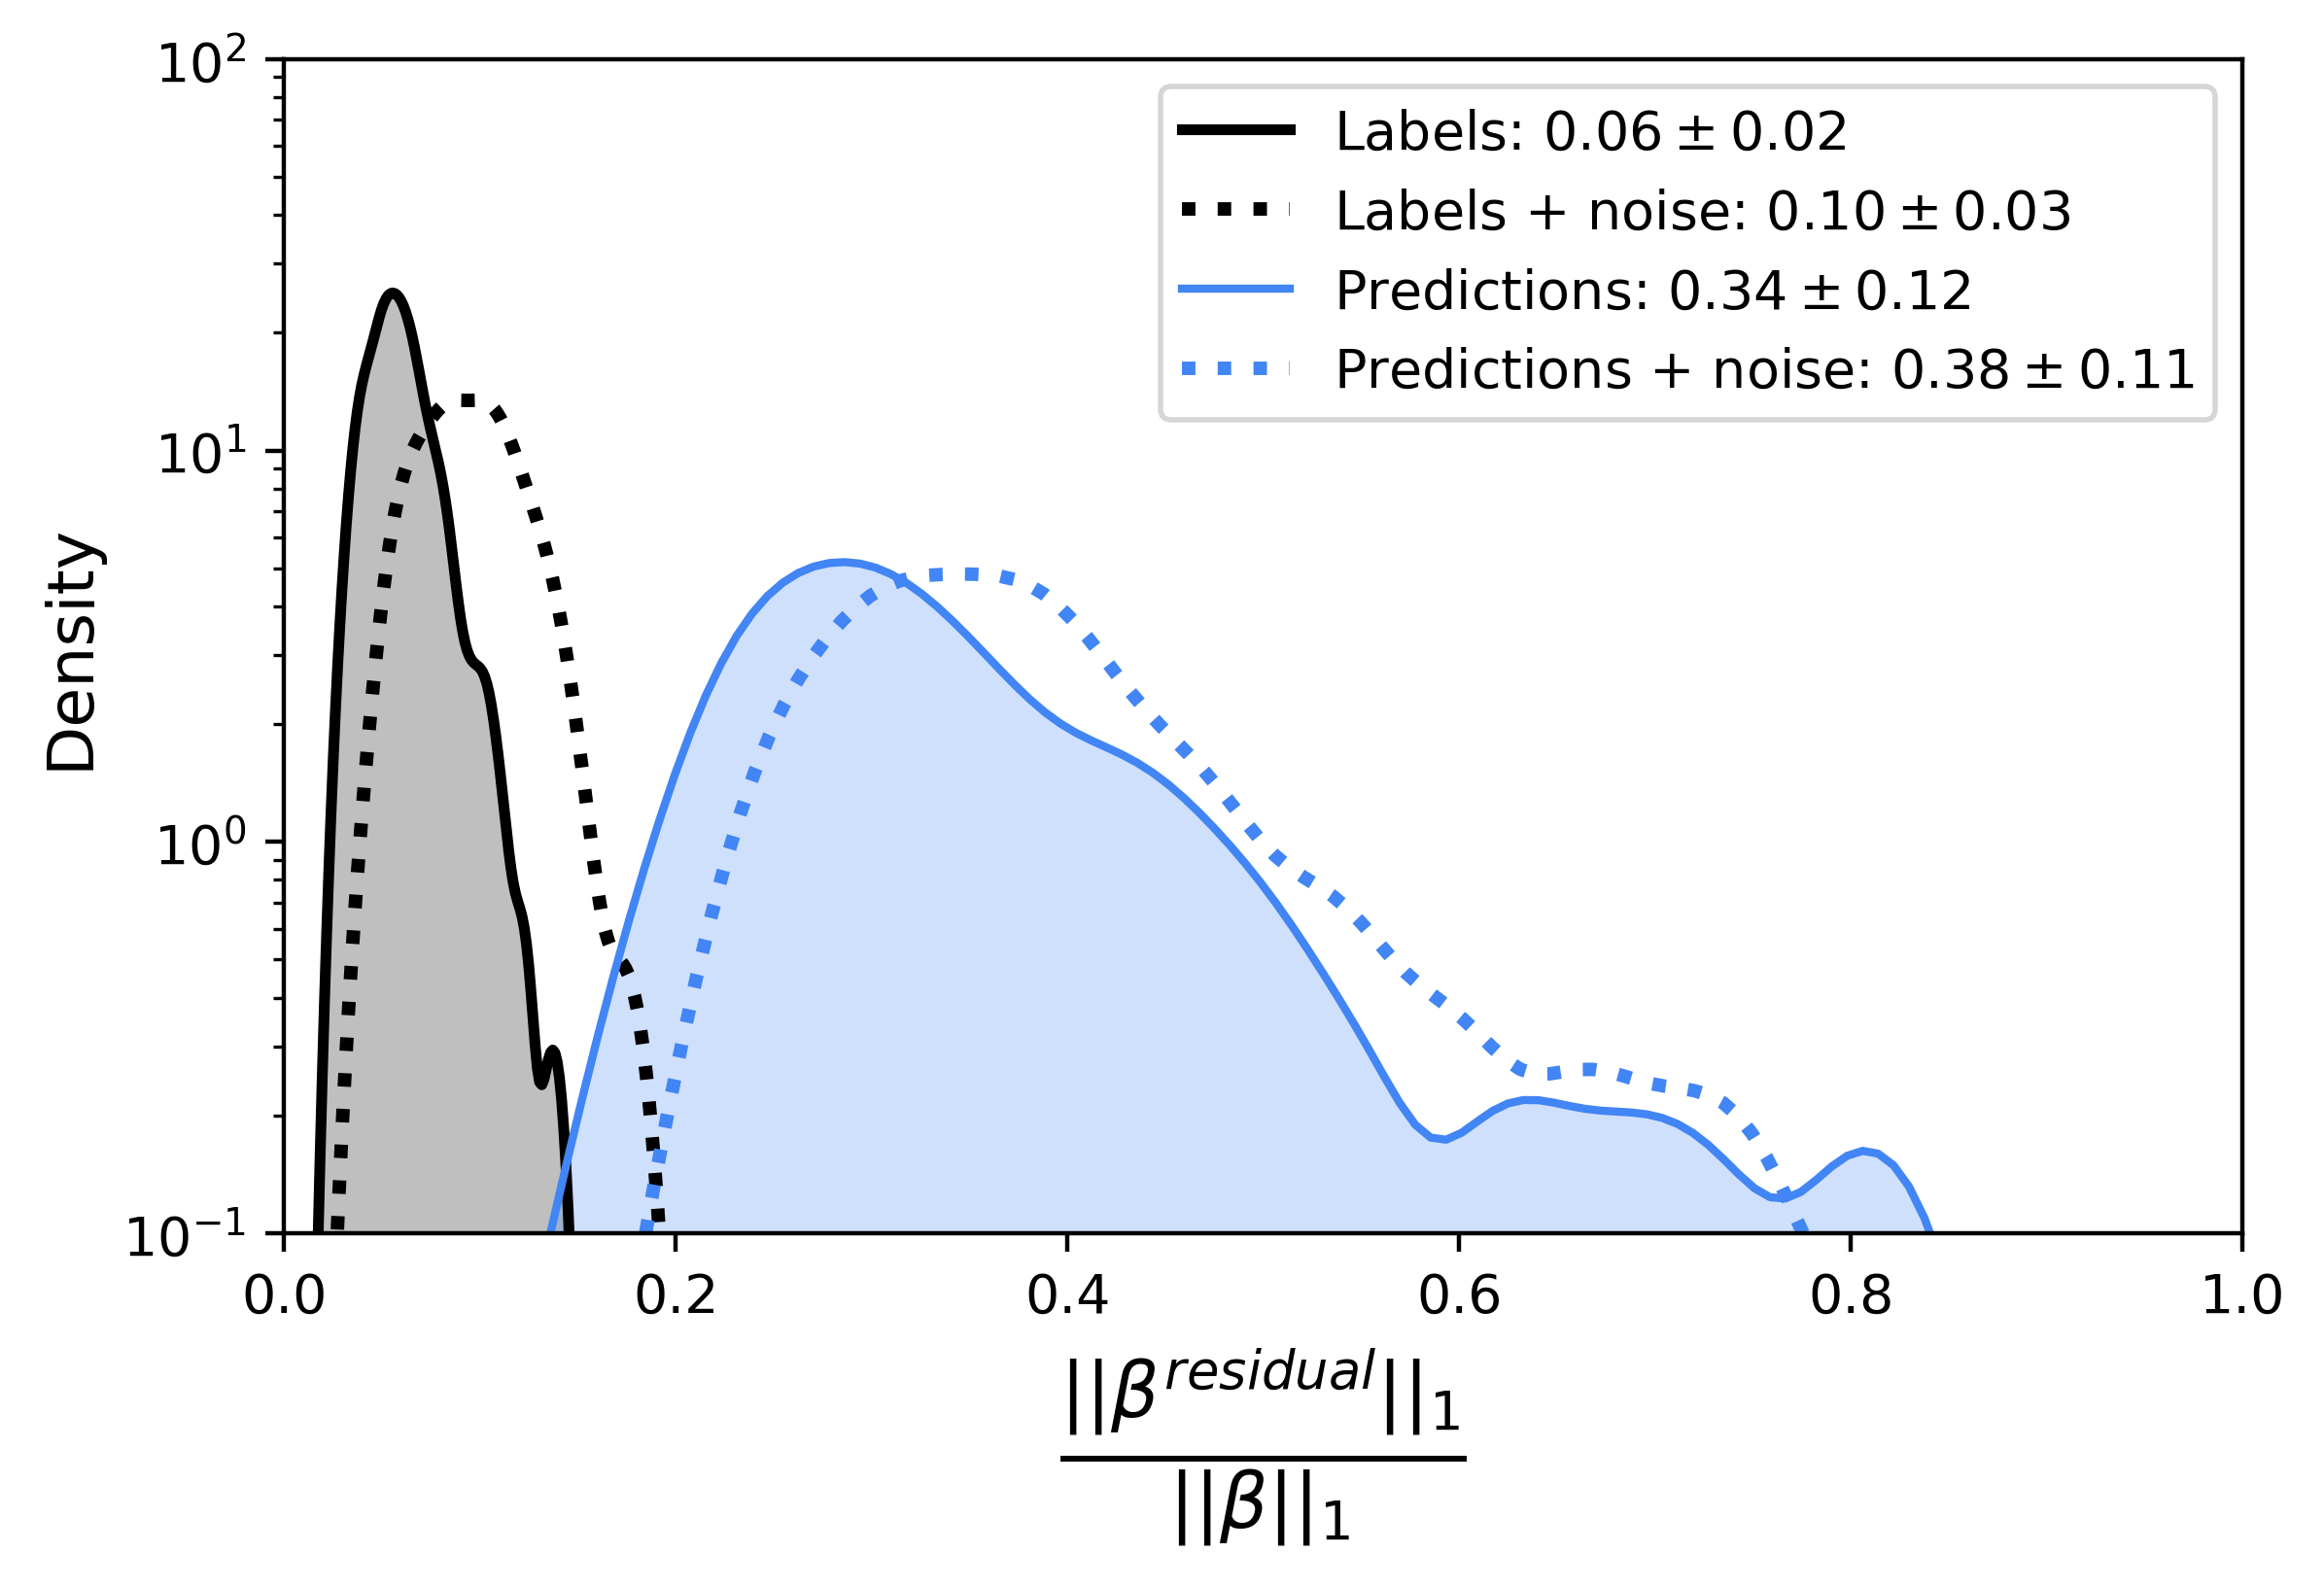
\includegraphics[width=\textwidth]{figs/interp/dist_defense2.png}
\end{tabular}
\end{center}
\caption[Relative Residuals In Different Scenarios]{The distributions of relative residuals in four different scenarios. The distributions from performing the interpolation over the labels with and without noise are shown in black. The distributions from performing the interpolation over the local wavefront predictions from the neural network with and without noise are shown in blue. \label{fig:beta-results}}
\end{figure} 

In the first scenario, we evaluated the second step of our algorithm on the true local wavefront labels from the first step. The relative residual is 6\%, which validates that our simulations are consistent and there are no sources of catastrophic numerical error. In the second scenario, we added uncorrelated Gaussian noise to each local wavefront coefficient. The variance of the noise for each coefficient was equal to the variance of the neural network error on that coefficient in the test data. Despite this noise, the relative residual remained very low at 10\%. This shows that our approach is not overly sensitive to uncorrelated noise.

In the third scenario, we fed the local wavefront predictions from the neural network to the second step. These have significant correlated error due to the atmosphere. The relative residual is 34\%, extremely promising, with a tight 12\% standard deviation. Furthermore, the right tail decays rapidly. Not a single relative residual is greater than one. Our framework improves the global wavefront on every observation in the full visit dataset!

In the fourth scenario we add noise as in the second scenario, effectively doubling the error. The relative residual increases slightly to 38\%. This suggests that the network is fairly robust to uncorrelated noise.

\section{Combined Runtime}

The run-time is another key advantage of our approach. It takes just under 4 seconds to process 811 donut images on a 2.4 GHz Intel Xeon CPU with a single Nvidia V100 GPU. It takes an additional 5 milliseconds to run the least squares optimization. The total processing time per donut image is 5 milliseconds; the total processing time per donut of the Rubin Observatory AOS under development is around 10 seconds\cite{2015Xin,2014Overiew}. Our scheme can process donuts 2,000 times faster, and is capable of processing 7,800 donuts in a single 39 second Rubin visit. The low latency allows it to process all the donuts in most observations.

\section{Image Quality Results}

The next step is to take this model and measure the repercussions of subtracting its estimate from the true wavefront on both the PSF FWHM and Strehl ratio \cite{strehl1895aplanatische}. We compute these by calculating the local wavefronts at the center and one corner of the focal plane. Then we take the fourier transform of the resulting pupil plane aberration to get the point spread function. The results for the original and corrected wavefronts are shown in Table \ref{tab:corrections}. 

\begin{table}
{
    \begin{center}
    \begin{tabular}{|l|l|c|c|}
    \hline
    State & Position & FWHM & Strehl\\
    \hline
    Before & Center & $0.288 \pm 0.034$ & $0.093 \pm 0.39$ \\
    After & Center & $0.211 \pm 0.005$ &  $0.555 \pm 0.207$\\
    \hline
    Before & Corner & $0.314 \pm 0.045$ & $0.074 \pm 0.32$\\
    After & Corner & $0.215 \pm 0.009$ & $0.400 \pm 0.184$\\
    \hline
    \end{tabular}
    \end{center}
}
\caption[Improvements To The Optics PSF FWHM And Strehl Ratio]{We measure the optics PSF FWHM and Strehl ratio on the original optics wavefront from the observation (Before), and the residual wavefront resulting from subtracting our wavefront estimate from the original optics wavefront (After). The Center position is at the center of the Rubin focal plane; the Corner position is at the center of the $R00$ wavefront sensor in the corner of the focal plane.}
\label{tab:corrections}
\end{table}

The optics PSF FWHM decreases considerably, especially when compared to the standard deviation of the original. The Strehl ratio increases in an even more extreme manner. Figure \ref{fig:vision} provides an illustrative example of how the improvements to the optics PSF from our method can improve image quality. We apply the Rubin optics PSF, before and after subtracting the optics wavefront estimated by our framework, to six classic Hubble Telescope images in the absence of other significant PSF contributions.

\begin{figure}[!htbp]
\begin{center}
\begin{tabular}{c}
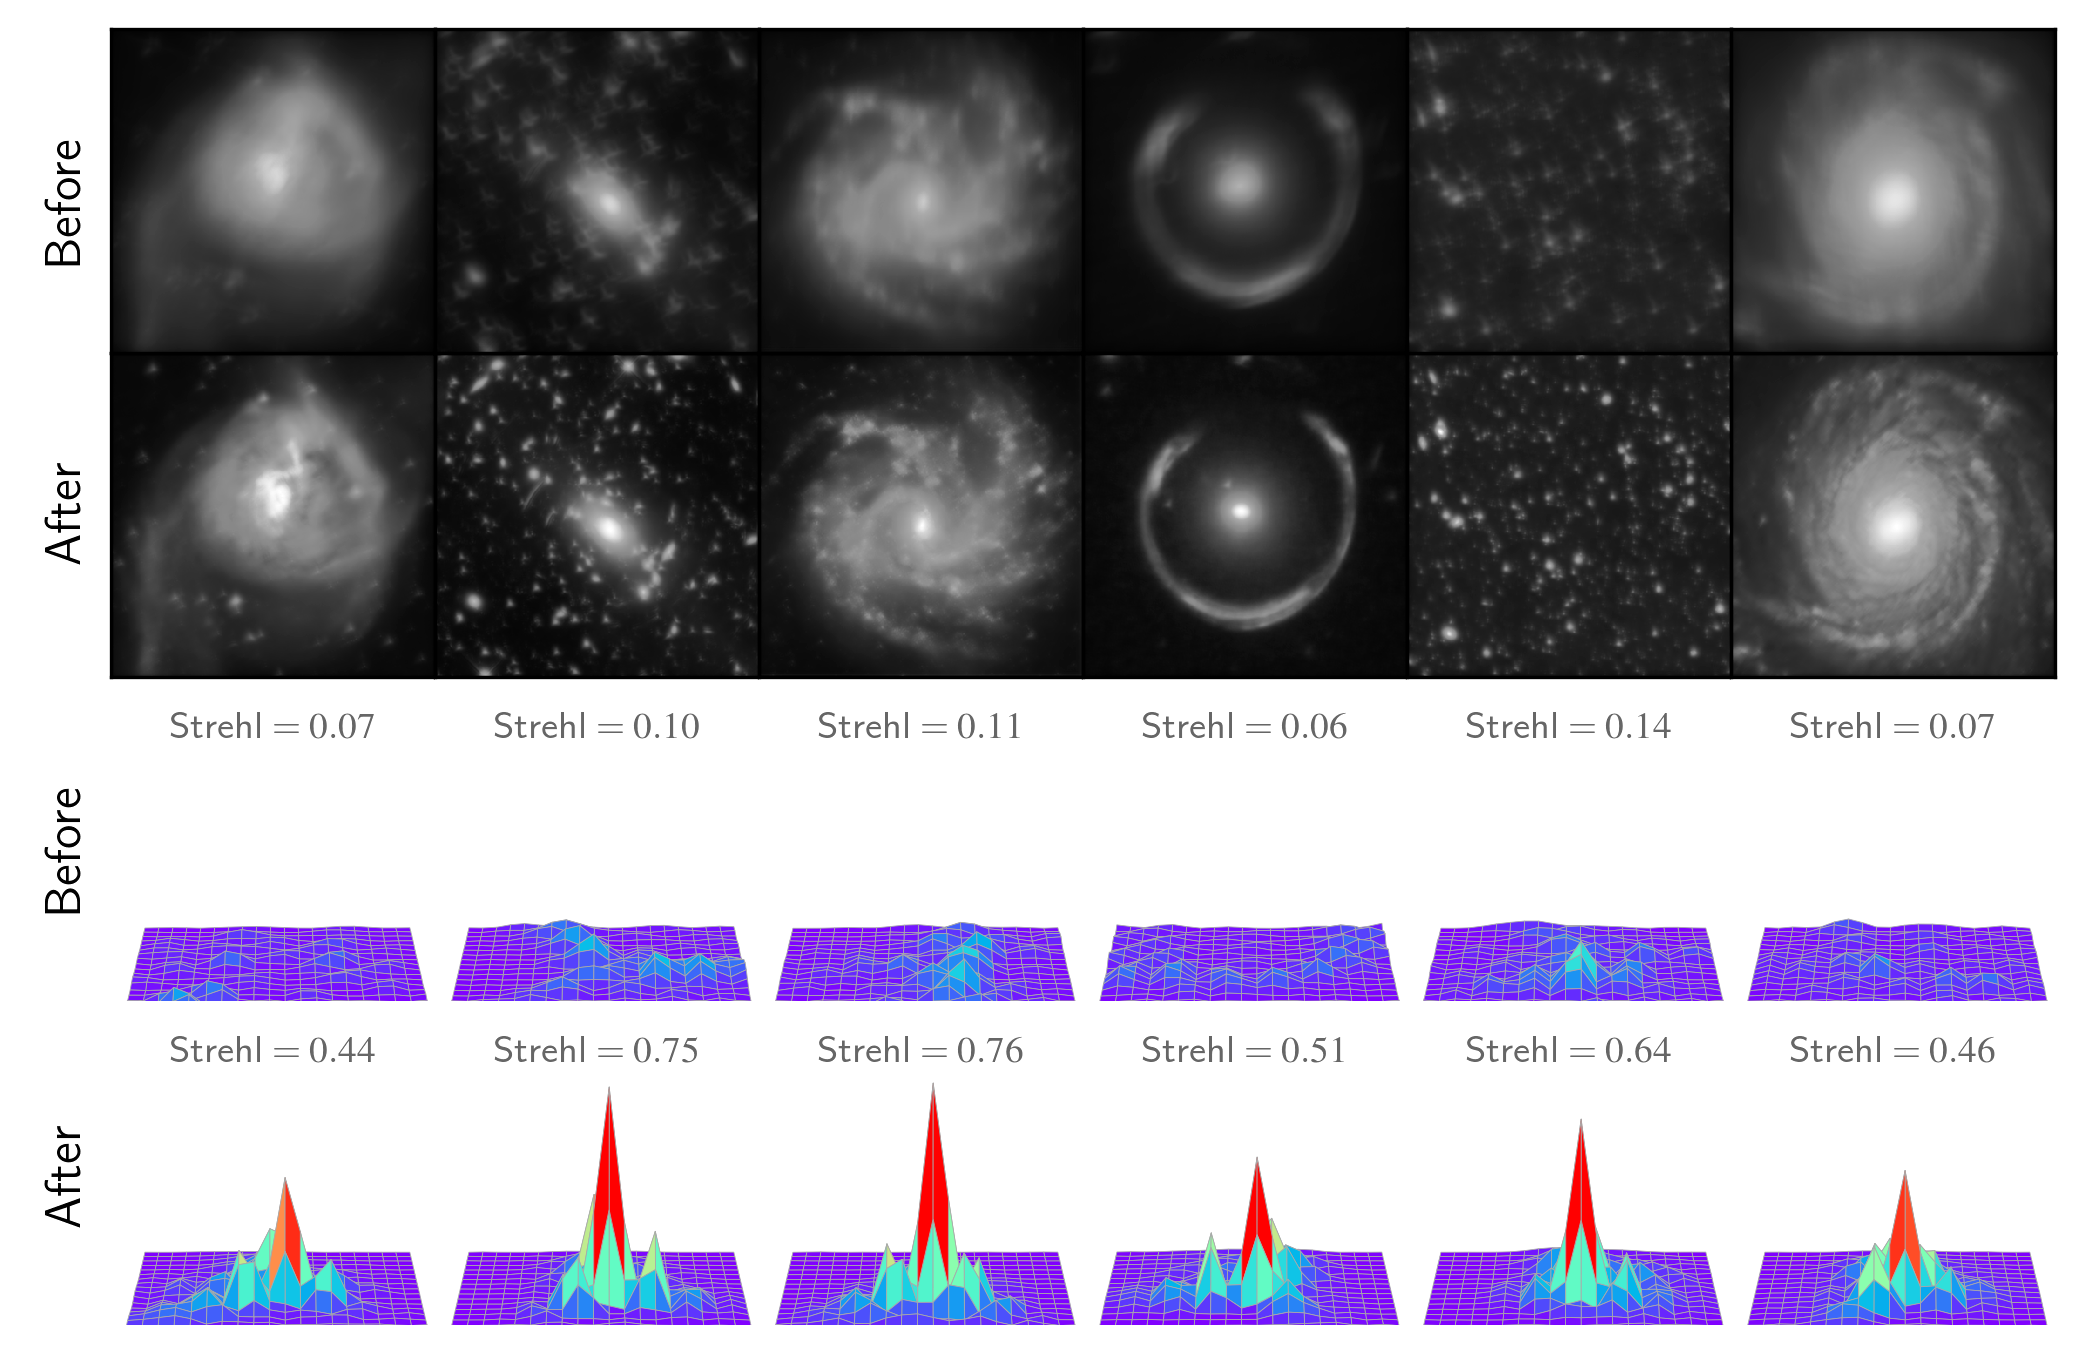
\includegraphics[width=\textwidth]{figs/interp/results.png}
\end{tabular}
\end{center}
\caption[Illustrative Hubble Telescope Images After Correction From Our Framework]{An illustration of the effect of wavefront correction using our techniques on image resolution.  We use actual Hubble Space Telescope images to show the effect.  The Before images are degraded by the wavefront aberrations we have simulated.  The After images show their reconstruction after wavefront estimation and correction using the technique we describe in this paper. On the bottom two rows, we show the effective PSF, both before and after wavefront correction. The images have an angular extent of 3 arcseconds and the PSFs are displayed on a $0.16 \times 0.16$ arcsecond grid. \label{fig:results}}
\end{figure}

For the Rubin Observatory however, the PSF is dominated by the atmosphere, which as indicated cannot be corrected. For the Rubin observatory the assumed PSF width is of order 0.71 arcseconds, of which 0.65 is contributed by the atmosphere. Therefore, the improvement in the Strehl and image quality is not as dramatic. Nevertheless, this improvement is still important for use on nights with unusually good atmospheric seeing and also for applications that are especially sensitive to the PSF width.
